\documentclass[12pt]{article}
\input{preamble}

\pagestyle{fancy}
\fancyhf{}

\rhead{Nørre Gymnasium\\
2.c
}


%Husk at rette modul og dato!
\lhead{Matematik B\\
Modul 1
}
\chead{12/11/2021
}

\cfoot{Side \thepage \hspace{1pt} af \pageref{LastPage}}

\begin{document}

%Udfyld afsnit herunder og lav til egen Latex-fil


%Overskrift
\begin{center}
\Huge
Differentialregning
\end{center}
\section*{Indledende knæbøjninger}
\stepcounter{section}

Differentialregning går lidt løst sagt ud på at se på hvordan "pæne" funktioner ændrer sig lokalt. Vi vil kun ganske uformelt diskutere, hvad der menes med pæne funktioner. Vi vil starte med at betragte et eksempel.
\begin{exa}
Vi forestiller os, at vi kører i en bil, og vi er interesserede i hvor stærkt, vi kører på et tidspunkt $t$. Lad os sige, at vi fra tidspunkt $t$ til tidspunkt $t+5$ måler, at vi er kørt $200m$. Så ved vi, at vi i gennemsnit har kørt med en hastighed på
\begin{align*}
\frac{200m}{5s} = 40\frac{m}{s},
\end{align*} 
men vi ved fortsat ikke, hvor stærkt vi kørte nøjagtigt ved tid $t$. Vi måler derfor, at vi til tidspunkt $t+2$ har kørt $70m$. Vi ved derfor, at vi fra tid $t$ til tid $t+2$ har kørt med en hastighed på 
\begin{align*}
\frac{70m}{2s} = 35\frac{m}{s},
\end{align*}
og vi kommer en smule nærmere den korrekte hastighed til tid $t$. Den korrekte hastighed må derfor blive tilnærmet mere og mere jo mindre tidsinterval, vi måler hen over bliver. 
\end{exa}
Inspireret af dette eksempel, vil vi definere den såkaldte differentialkvotient, der fortæller noget om den øjeblikkelige tilvækst af en funktion. 
Betragt funktionen på Fig. \ref{fig:sek1}
\begin{figure}[H]
\centering
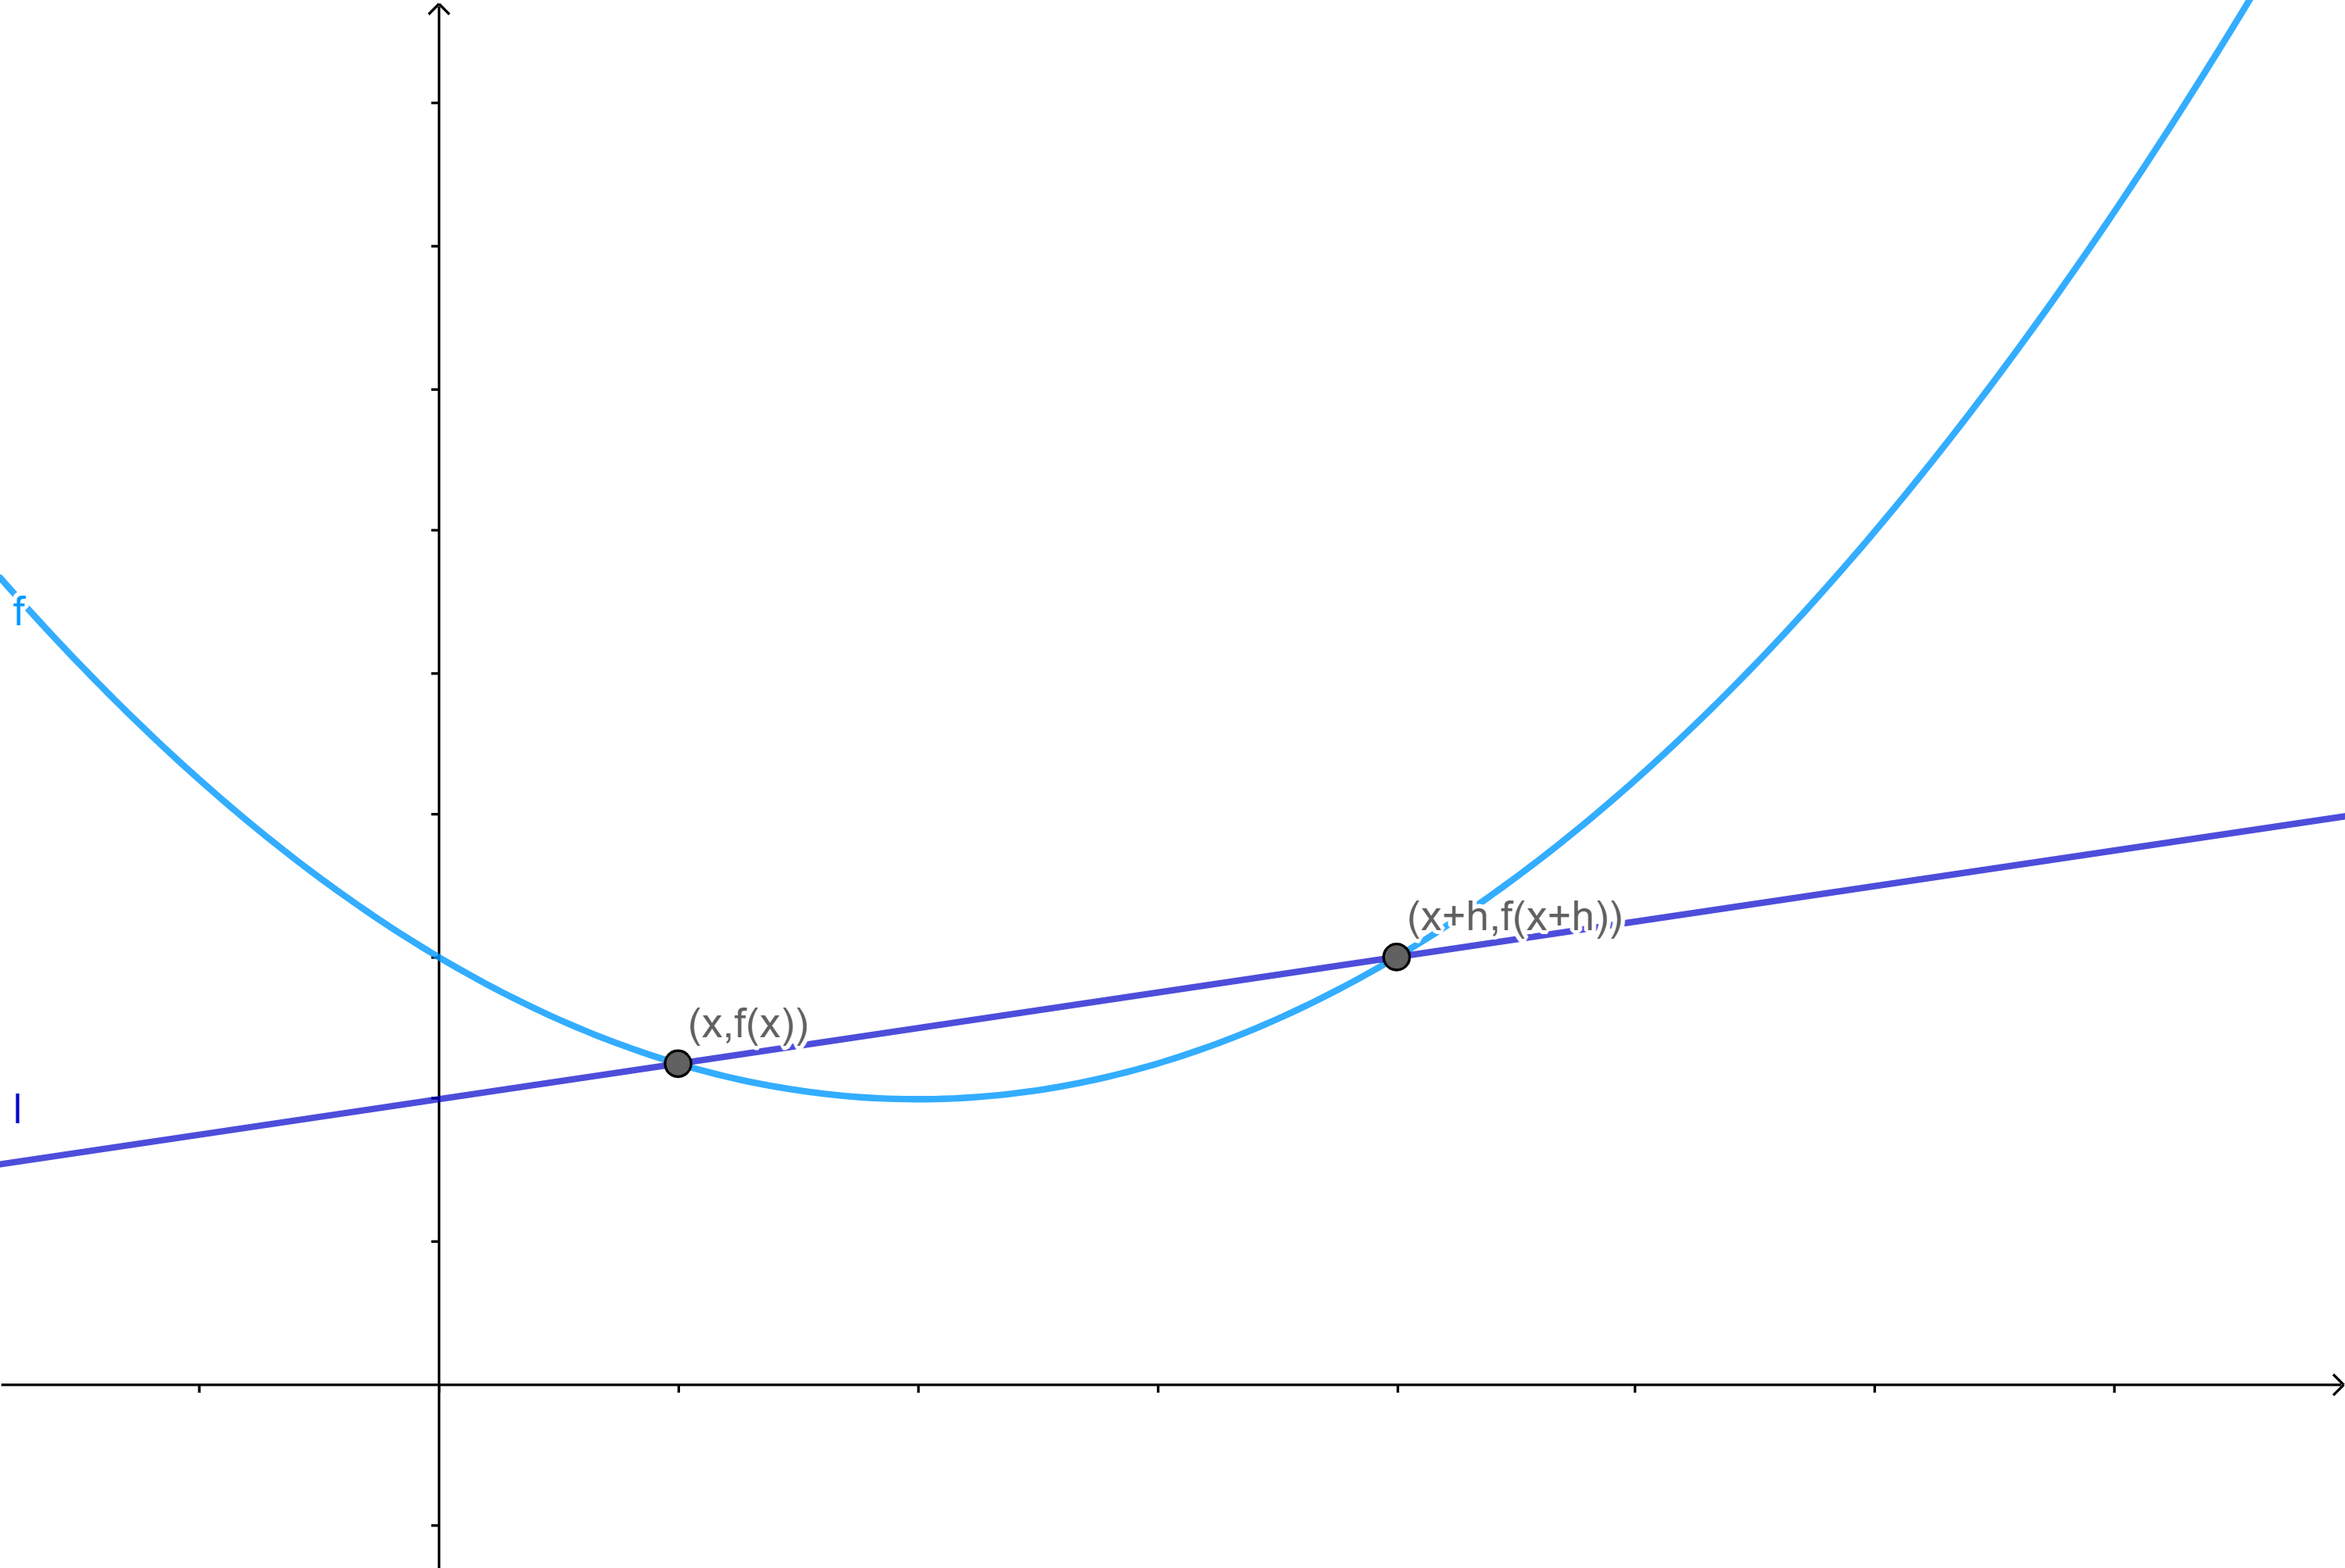
\includegraphics[width = 12cm]{Billeder/sekant1.png}
\caption{Funktion med sekant gennem punkterne $(x,f(x))$ og $(x+h,f(x+h))$.}
\label{fig:sek1}
\end{figure}
\end{document}
